
\documentclass[10pt,conference]{IEEEtran}

\usepackage{url}
\usepackage{graphicx}

\hyphenation{}

\begin{document}

\title{Social Footprints : Public Profile Attributes to Determine User Vulnerability in Online Social Networks}

\author{\IEEEauthorblockN{Hamza Karachiwala\IEEEauthorrefmark{1},
Kedar Amrolkar\IEEEauthorrefmark{2} and
Mickey Vellukunnel\IEEEauthorrefmark{3}}
\IEEEauthorblockA{
University of Florida\\
Email: \IEEEauthorrefmark{1}hskarachiwala@ufl.edu,
\IEEEauthorrefmark{2}kamrolkar@ufl.edu,
\IEEEauthorrefmark{3}m.vellukunnel@ufl.edu
}}

\maketitle

\begin{abstract}
Social networks have been a very important advance over the last decade and a half. Today, there are various types of Online Social Networks or OSNs. Most of these OSNs have a very large user base which confirms their popularity and also their need in the present time. These users tend to disclose much of their identifying information on these sites via public profiles in order to be discovered by other users. However, these users may also be malicious and pose a threat to others in the network by collecting public profile data of any user. While there may not be enough public data on a single OSN, the public data across all the OSNs aggregated together results in a comprehensive collection of user profile data. This aggregated data is called a social footprint. We intend to measure how heavy a users aggregated footprint may be, given the user has accounts on different Online Social Networks. We measure this by assigning weights to all the individual public profile attributes that build this footprint. These weights are assigned based on the sensitivity and the need of having a particular attribute disclosed in a user's public profile. We then identify if the aggregated weight of this footprint crosses a threshold value making it vulnerable to a malicious attacker. If the footprint is vulnerable, we suggest possible ways of reducing the weight of this social footprint.
\end{abstract}

\section{Introduction}
We have witnessed the advent of various social networking sites over the last decade and a half. And along with this, we have also witnessed the phenomenal adoption of these social networks. Users on these sites continue to multiply daily, which highlights the willingness of the masses to join this OSN bandwagon. Statistics show\cite{statswebsite} that the number of users worldwide has increased from 0.97 billion to 1.96 billion in just the last five years. This number is expected to shoot up to 2.5 billion by 2018. In fact, another striking statistic is that 75\% of the US population has a social network profile. Which means that 3 out of every 4 people can be found online. These statistics are not only restricted to a single age group or income group, but are in fact applicable to a wide range of audience as can be observed from \cite{secondstat}. It is safe to say that social networks have definitely been a very influential advance in computing and the numbers and statistics listed above corroborate that.\\

Moreover, these sites cater to different aspects of our lives. One would often have separate social networks for his personal and professional lives, a separate platform for photo sharing and at the same time, a public channel for videos. These social networks that are ever evolving, continue to be more and more pervasive in our lives. Although this remarkable progress is highly commendable, it does come with its own perils. After all, it is a ``social'' network with humans communicating with each other. While providing a rich source of both information and interaction, it also requires us to disclose some basic facts about ourselves such as our name, gender and in some cases our photograph. The purpose behind disclosing these attributes is so that a user can be ``visible" on the network. That is, a user can be discovered or recognized from the others on a network. However, while this visibility information can be bare minimum, we sometimes unwittingly disclose information about ourselves on these websites which would actually be quite sensitive or private. While we see it as a little bit of information about ourselves, these bits and pieces spread over varying social networks aggregated together as illustrated in \cite{privacypaper}, makes it possible for people with malicious intent to gain information about us which may be used in a harmful way. While the independent bits and pieces of information may be harmless by themselves, a systematic collection of all that data paves the way for various crimes such as identity thefts, dictionary attacks, harrassment, etc\\

Consider this report \cite{newsarticle} from 2014 which dishes out a few astonishing numbers related to cyber crimes. In the surveys conducted, it was found that 78\% burglars used the geotagging features across OSNs to locate their victims and plan their strikes. Almost 50\% of sex crimes committed against a minor involves the perpetrator obtaining profile pictures. But here is the most worrying statistic - 66\% of Facebook users had no notion of what privacy settings were and what they had disclosed online. 15\% also admitted that despite the knowledge, they never bothered to check because there are so many sites. This illustrates the carelessness of the masses in general when it comes to protecting profile data. And while this may not be as harmful on a single OSN, or the dangers might not be highlighted by a limited number of attributes, the problem magnifies when we pick data from multiple OSNs and build a social footprint by aggregating all this data. The amount of disclosed data increases drastically. Subsequently, it increases the vulnerability or susceptibility of a user to attacks that can be carried out by knowing that information.\\

Our aim is to warn users about the risk they may be exposed to because of this level of information disclosure in cyberspace. By accessing various degrees of their data on these social network websites, we want to build an aggregated profile of a user - his social media footprint, along similar lines as explained in \cite{emergingthreat}. This social media footprint will be an intuitive metric of an individual’s presence across social networks. We want to further provide this footprint to a user with the intention of encouraging him to trim down the personal information he might have disclosed. Users are often not aware of the consequences and through this work, we can generate that awareness. While various surveys have been conducted over the same concerns, there have been no known attempt to formalize the vulnerability of a social footprint. It is of prime importance to reach out to users and explain this hard-to-visualize problem in a simplistic and intuitive way.

%give more detail in related work
\section{Related Works}
Researchers have since long identified the need for privacy in social networks. They have studied the implications of leakage and the consequences as also suggested methods to avoid this \cite{emergingthreat},\cite{inforevelation},\cite{privacypaper},\cite{undermining}. Moreover, they have observed that while it is risky to disclose information on an OSN, that is also the base of its success. In order to gain the benefits of an OSN, it is necessary to share certain information and be identifiable to a certain set of people at least. This is the reason that makes it important to study footprints and aggregated data as proposed in \cite{emergingthreat},\cite{leakage} and \cite{paas}. Various proposals have been made to calculate an aggregated footprint on a single website or spanning multiple sites and then measure the risk associated with these footprints \cite{socialgraph},\cite{framework}. These methods rely on intuition to weigh leaked profile attributes. We will attempt to provide weights by studying past crime instances that occurred as a result of attribute leakage. For example, a burglary that is caused by a checkin would mean a higher weight for a checkin. Or accounts are hacked due to dictionary attacks. These dictionaries are created using profile data and something like a school name would possess a higher attribute weight if a crime has been carried out by using it. \\

However, there has been a marked rise in the number of OSNs since the past few years. And most of these OSNs have not been included in the various analyses and works done above. While the core contributors to a social footprint would remain very much the same, there are some interesting new attributes that are now added to a social footprint. These are worth investigating as well. Namely, interest lists that may be garnered from Pinterest or favourite public figures that may be enlisted from Twitter. These lists can be used for other activities such as targeted advertisements which would in a way be illegal as that profile data is not meant to be used.\\

There have also been some interesting and in depth mathematical models designed which we would be interested to incorporate in our analysis. The represenation by Irani et al \cite{leakage} of a social footprint as \(\tau_{s}^{u}\) is very intuitive. They then create an aggregate represenation \(P^{u}=\bigcup\tau_{i}^{u}\) for the footprint spanning various sites. Another notable mention is the {\sl PIDX} proposed by Nepali et al. \cite{pidx}
\begin{equation}
PIDX(i,j) = \frac{w(i,j)}{w(j)}\times100
\end{equation}
While there are tools proposed to analyze data on Facebook \cite{privometer} and \cite{privaware}, we are attempting to provide a common application for thorough footprint measurement. Privometer was especially promising as a Facebook app which uses a smilar procedure to calculate the weight of public profile infrmation disclosed on Facebook. It also had some self explanatory graphic interfaces for the user to help him understand the dangers of disclosing this data and how these dangers could be averted by minimizing some of the data disclosed on the public profile. However Privometer is not available as of today for use and some of the Facebook regulations have changed over time. While Facebook is undoubtedly the major contributing factor to a footprint, the aggregation from multiple sites is what largely includes the risk element. We have access to more of these OSNs via APIs than it was possible before, with the advent of REST architectures in the web industry.

\section{Problem and Solution}
In this section, we identify the scope of our problem and then illustrate our approach to solving it. Our main aim is to generate awareness among OSN users about the concept of social footprinting. While a user may be aware of the risk of disclosing information on a single OSN, he would most probably not be aware that profile information across multiple OSNs can be aggregated to generate a more comprehensive list of user information. As mentioned in \cite{emergingthreat}, while a user may disclose 4 unique fields in a single OSN, this number doubles when he/she is a user of five OSNs. This information can then be exploited by miscreants and criminals to cause harm to the user. This may range from offences such as harassment or stalking to crimes such as identity theft. \\

To solve this problem, we first need to collect aggregated data from a user spanning across his multiple social network accounts to build his social footprint. We will achieve this using the APIs exposed by these OSNs. Most OSNs provide these APIs to integrate with other applications. In the case of Facebook, LinkedIn and Google+, they also act as an authentication medium. We will use this functionality to fetch user data from these three websites and avoid the cumbersome crawling or scraping data from these websites for a user. While Facebook and Google+ are complete social networks in a sense, LinkedIn is restricted to professional data. Together, we believe that these three sites would cover a majority of common public attributes and would make quite an accurate social footprint, if not the most accurate. We will discuss some other sources of data in Section 5 and how they could improve on the comprehensiveness of the footprint. The remaining of this work, however, uses Facebook, Google+ and LinkedIn.\\

Once we have built a footprint, we need to measure its weight. In order to do this, we must have weights associated with all the attributes of a user's profile data. We will be assigning these weights based on statistics related to two kinds of attacks - and password recovery. We propose to assign these weights based on empirical estimates derived from criminal records, census and survey information. We will list out which attributes contribute the most toward crimes caused by data leakage via public profiles. For password recovery, we build on the work of Bonneau et.al \cite{google} which highlights the risk of using password recovery questions. In both cases, the idea is to assign a higher weight to an attribute that is associated with more risk, or could be more harmful to divulge as part of the footprint. While the statistics we have to back our mathematical model are limited, we believe that it is trivial to strengthen these claims and would simply need some more work on data collection. We explre this in detail in Section 5. \\

Based on the weights assigned to attributes, we will compute the aggregated weight of the social footprint. This weight can be calculated trivially as the sum of the weights of all the attributes that have aggregated into the footprint. Then comes the challenge of identifying the risk associated with that footprint. We need to identify a threshold value beyond which the weight of a social footprint would classify as at-risk. We intend to assign a simple average value for this due to the time constraints. We will assume for now that a name and profile picture is a bare minimum requirement for visibility in these sites. Our threshold will be 
\begin{equation}
w(first-name) + w(last-name) + w(profile-pic)
\end{equation}
where \textit{w(.)} is the weight assigned to any attribute. This is the simple weight required by any profile to be visible or discoverable in the least. We will consider any other information above this as associated with some risk. We propose improvements to this approach in Section 5. Following this, our next task will involve identifying ways to reduce the weight of a social footprint. In this step, the user will be suggested various attributes that could be left out or hidden from his public profile. The objective will be to minimize the footprint weight by leaving out heavy attributes that would be associated with most risk. While we would like to find an optimal subset of attribute weights that maintain a balance of visibility and risk, in this work we restrict our suggestions to a greedy approach that suggests pruning attributes in decreasing order of weights.\\

In the following subsections, we give details on each of these steps required to solve this problem by outlining the approach and the obstacles that have to be overcome to improve this approach.

\subsection{API Integration}
The technology stack that we use for the web application is Apache as the server, PHP for the server side scripting and MySQL as the database. PHP is the choice language to integrate with these OSNs via APIs as all of them provide comprehensive documentation to integrate with their services. Also, these technologies being Open Source is a contributing factor in using them. The authors do not have prior experience with PHP which is a significant challenge. The MySQL database can be used for historic data and statistic collection. However, our web interface does not require interactions with the database. Figures 1 and 2 illustrate the use of the interface. A user will access the web application and then provide his authentication for the three OSNs that he uses. This is needed to call the API to fetch that users data. We do not store his login credentials in any way and simply use the third party authentication service provided by these three OSNs. The user is then prompted for permission to access his public profile. On providing this permission, the user allows us to view his public profile attributes. We then build a union of attribute lists of all the three OSNs. This would adhere to the definition of social footprint that we mention in the previous section. Table 1 lists attributes and the OSN they can be retrieved from. We have built this list manually and may not be exhaustive.

\begin{table}
	\normalsize
	\centering
 		\begin{tabular}{|| c | c ||} 
 		\hline
 		Attribute & Source\\  
		\hline\hline
		First Name & Facebook, Google+, LinkedIn \\
		\hline
		Last Name & Facebook, Google+, LinkedIn \\
		\hline
		Profile Picture & Facebook, Google+, LinkedIn \\
		\hline
		Gender & Facebook, Google+, LinkedIn \\
		\hline
		Date of Birth & Facebook, Google+, LinkedIn \\
		\hline
		Email & Facebook, Google+, LinkedIn \\
		\hline
		Phone number & Facebook, Google+, LinkedIn \\
		\hline
		Marital status & Facebook, Google+, LinkedIn \\
		\hline
		Lives In & Facebook, Google+, LinkedIn \\
		\hline
		Previous cities & Facebook, Google+, LinkedIn \\
		\hline
		Works at & Facebook, Google+, LinkedIn \\
		\hline
		Occupation & Facebook, Google+, LinkedIn \\
		\hline
		Studies at & Facebook, Google+, LinkedIn \\
		\hline
		Previous work & Facebook, Google+, LinkedIn \\
		\hline
		Previous education & Facebook, Google+, LinkedIn \\
		\hline
		Family & Facebook, Google+ \\
		\hline
		Checkins & Facebook \\
		\hline
		Nickname & Facebook \\
		\hline
		Life events & Facebook \\
		\hline
		Projects & LinkedIn \\
		\hline
		Courses & LinkedIn \\
		\hline
		Skills & LinkedIn \\
		\hline		
		Circles & Google+ \\
		\hline
	\end{tabular}
\caption{List of attributes in a social footprint}
\end{table}

One observation that we can make here is that while some of the attributes at the bottom of the table are unique to some of the sites, a majority of the attributes are common to the three sites. This reinforces our motivation of a user accidentally leaking a comprehensive profile across various sites. While a user might be careful of protecting attributes on one site, it is extremely likely that the user may have leaked that same attribute information unintentionally on another site. This is how a social footprint might be exploited. We will revisit some of these possibilities in Section 4.

	\begin{figure}[h]
		\caption{Facebook Login Page}
		\centering
		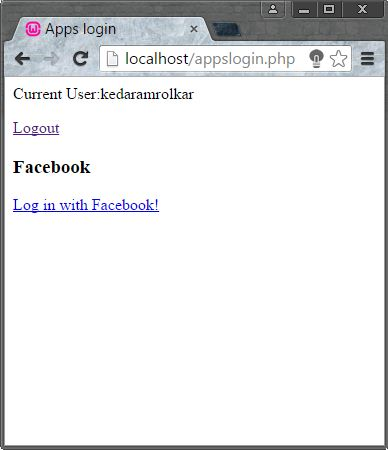
\includegraphics{loginfB}
	\end{figure}
  
	\begin{figure}[h]
  		\caption{User Data retreived from Facebook}
		\centering
		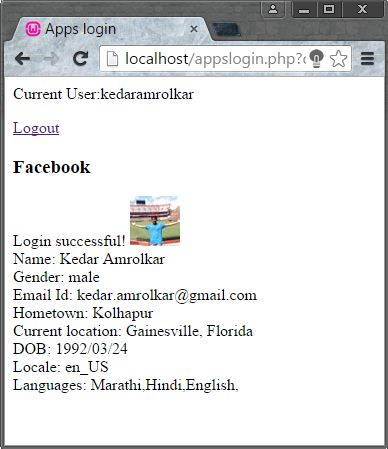
\includegraphics{fBdata}
  	\end{figure}

\subsection{Weight assignments}
We would like to assign weights to attributes based on the risk associated with divulging that attribute. Prior works assign these weights based on intuition which rely on the same idea. We propose that these weights should be based on how the attribute disclosure has already harmed users historically or statistically indicate that users could be harmed by disclosing that attribute. That is, we infer that attributes that are risky are the ones that can be used to harm the user in some way. The information held by those attributes would be of some private value and divulging them would not be safe for a user. Now, depending on the extent of the harm that may be caused by divulging an attribute, we give a weight to that attribute. In short, an attribute which, by being divulged in public causes more harm to a user, has a higher weight than the others. \\

We now talk about what can come under the definition of harm. As mentioned in the previous section, various crimes are tied to online social networks. Attackers use different tools, one of which is the use of information available on social networking sites. We explore two possible attacks - identity theft and password recovery.

\subsubsection{Password Recovery}
Most websites require users to create accounts. This provides a certain level of personalization with a user. On creating an account, the user chooses a username for the website and a password which would serve as his login credentials. However, passwords can be lost or forgotten. And moreover, in this age when there are so many different websites each requiring their own login, users tend to forget passwords often. According to statistics in \cite{passwordstats}, 80\% people have forgotten passwords at some point. Also, close to 60\% survey participants admitted to having the same password. This shows the need to have password recovery mechanisms. For this reason, many sites provide a mechanism to retrieve a password. In this process, users are asked to choose a security question, an answer of which would only be known to them. These questions are a general popular set apppearing across various websites. Table 2 shows a list of some popular security questions. 

	\begin{table*}[t]
	\normalsize
	\begin{center}
 		\begin{tabular}{|| c | c | c ||} 
 		\hline
 		Security Questions & Possible Answer Attribute & OSN \\ 
		\hline\hline
		Mother's maiden name? & Family & Facebook, Google+ \\
		\hline
		City of birth? & Previous City & Facebook, Google+, LinedIn \\
		\hline
		Name of wedding reception venue? & CheckIns & Facebook \\
		\hline
		Person you first kissed? & Relationshup Status & Facebook  \\
		\hline
		Manager at first job? & Projects & LinkedIn \\
		\hline
		Name of primary school? & Education & Facebook, Google+, LinkedIn \\
		\hline
		Where does sibling live? & Family $ \rightarrow$ Current Location & Facebook, Google+, LinkedIn \\
		\hline
		Vehicle Registration Number? & Life Event & Facebook \\
		\hline
		Pets Name? & Photos / Updates & Facebook, Google+ \\
		\hline
		Year Father was Born? & Family $ \rightarrow$ DOB & Facebook, Google+ \\
		\hline
		Favourite restaurant? & Check In & Facebook \\
		\hline
		Make of first car? & Life Event & Facebook \\
		\hline
		High school mascot? & Education $ \rightarrow$ Online search & Facebook, Google+, LinkedIn \\
		\hline
		Favourite Actor? & Likes / Interests & Facebook, Google+ \\
		\hline
		Favourite Musician? & Likes / Interests & Facebook, Google+ \\
		\hline
		Library Card Number? & - & - \\
		\hline
		First Telephone Number? & Phone & Facebook, Google+, LinkedIn \\
		\hline
		Childhood best friend? & Friends $ \rightarrow $ Check among all & Facebook, Google+ \\
		\hline
\end{tabular}
\caption{Security questions and possible answer attributes}
\end{center} 
\end{table*}

The arrow between attributes signifies a second step needed to reach an answer. As shown in the table, which is a list of popular questions, almost all questions can be answered by an OSN profile attribute. So we can now outline the attack method. An attacker who would want to break into another user's account would need to guess the password. Instead of guessing the password, an attacker can simply invoke the the recovery mechanism and attempt to answer the security question. A famous example is the Sarah Palin case where the attacker simply answered security questions from social footprint attributes. Examples of fields used in password recovery questions are mother’s middle name, high school name, etc. Existence of any one of these fields in a social footprint is enough to compromise the online account. \\

In order to assign weights to attributes keeping in mind the password recovery attack, we will use a recent survey paper by Bonneau et.al \cite{google}. This paper closely surveyed the current state of password recovery questions and concluded that this mechanism is not reliable. They also briefly explore the attack avenue outlined in our work but not in detail. In the process of their work, they carried out extensive surveys related to password recovery questions. Along with this, another major source of our statistics is the work of Rabkin \cite{recovery}. Rabkin has provided some information on 200 sample password recovery questions. While the motivation of his work was different, we can nevertheless make use of the numbers aggregated in his work. Some of the important statistics that we will use are -
 
 

\section{Roadmap for remaining work}
\subsection{Assigning attribute weights}
\paragraph*{Cross-site identifiers}  These are fields which on their own useless, but could be used to match profiles of a single user across multiple OSNs. For example, actual user profile pictures. If a user publically exposes actual pictures of himself, that along with another attribute (like name), could easily be used to find and identify his account on another OSN. Another example is when, on their own, gender, age and location might be benign, but when combined with name, it can be used to get info about the user from multiple OSNs to create a more complete social footprint. Also, country, birth year, sex and name (last name would be given more weight).\\
We do not have a timeline for weight assignments and will continue altering our weight table as we keep working with test footprints. If we do find a consolidated data souurce for crime history, it will expedite the process and we can prepare the table more easily. However, while we keep scanning bits of online resources, we cannot assign weights directly as different surveys are conducted with different external factors affecting them. Also they are conducted among different groups - for example, sex crimes in Mexico should be analyzed differently from identity thefts in Russia. Both these crimes require different subsets of a footprint and the weight table should be altered accordingly.
\subsection{Calculate and compare with threshold}
After having a list of assigned values for different attributes, we then calculate the weight for that user's footprint. We must check what attributes are present in the user's footprint. According to that we will fetch those attriute weights and do a simple sum on those weights. This will amount to the total weight of that footprint.
Mathematically, this can be represented as,
\begin{equation}
w(footprint) = \sum_{i=1}^{n}attribute_i
\end{equation}
\subsection{Check for vulnerability}
After we calculate the weight of the footprint, we compare it to a threshold value to check if it is vulnerable. We plan to do this simply by considering the average footprint weights of five users who can be considered to have safe footprints. That is, these users will be having very minimal public profile attributes which guarantee bare minimum visibility on these websites. This average footprint weight will be considered as the threshold for our remaining checks. While this is crude as compared to some previous works as in \cite{pidx}, it will temporariliy accomplish the requirements and we can extend on this approach when time permits. We intend to prepare the threshold value three weeks from this submission as we need all the API integrations before verifying with the safe footprints.
\subsection{Suggestion reduction in weights}
Once we have the threshold value and the result of the comparison with that value, we can determine the vulnerability of the footprint. In simple words if the footprint weight crosses the threshold value, it is vulnerable and we must bring the footprint weight down below the threshold. In order to achieve this, some attributes need to be removed from the users footprint or effectively from their OSN profile. This must be done keeping in mind that visibility must not be reduced drastically. We need to minimize the weight of the footprint and at the same time keep the visibility constant. While this is a classic linear programming problem, we will simply provide suggestions to users in decreasing order of weight of attributes. Considering that the weights will be assigned keeping in mind visibility, we can assume that heavy attributes will also be ones that will be affecting visibility less. The user can then decide if he wants to modify his profile or not. We will only provide suggestions.

\begin{table}[!t]
\renewcommand{\arraystretch}{3.0}
\caption{Attribute Weights (Single) based on Crime Records}
\label{attribute_table}
\centering
\begin{tabular}{|c||c|}
\hline
\large{First Name} & \large{2}\\
\hline
\large{Middle Name} & \large{1}\\
\hline
\large{Second Name} & \large{5}\\
\hline
\large{Age} & \large{1}\\
\hline
\large{Sex} & \large{1}\\
\hline
\large{Mothers Maiden Name} & \large{10}\\
\hline

\end{tabular}
\end{table}

\section{Results and Analysis}

\section{Future Work}
There is much scope for improvement in our approaches which would demand more time and statistical resources. While we have integrated with Facebook, Google+ and LinkedIn, there are many more OSNs which would be worth investigating in terms of attributes. Twitter, for example, is another example of a very popular social networking site and works on a different dynamic. One would, however, argue that the public profile attributes remain the same across these OSNs. While this is true, certain sites may contain specific content that could be more helpful towards profiling. Politicians followed on Twitter, music preferences on SoundCloud, artistic interests on Pinterest, image content on Instagram, video content on YouTube, etc. are some examples of OSNs that cater to very specific kinds of content. In some cases the entire profile content may be public, which makes the user very vulnerable to profiling and social engineering. These avenues are interesting to explore for this reason. Consequently, all user content is visble to connections on a site. By connection, we mean a friend on Facebook or a circle member on Google+, etc. We assume these connections to be trustworthy, but in the event that a connection is malicious, it gives the attack an entirely different magnitude of potency.\\

For our weight assignments, there are possible improvements as also different approaches that we may take. While we currently do consider password recovery attacks, in the near future it is likely that such question based systems will be obsolete \cite{google}. Even within the weight assignments for password recovery attacks, we could collect more data related to security questions such as a larger question set and question popularity in order to make our assignmets more accurate. In terms of safety threshold, we have a trivially defined value in our system. If we focus on the tradeoff between risk and visibility, we currently have not worked on formalizing visibility in the same way as risk. Hence, it is essential to be more accurate to decide if an attribute is required for visibility or if it should be considered risky. In order to understand that, we would need to perform more experiments and conduct more surveys to understand the visibility requirement in a public profile. On gaining more knowledge about visibility, we could come up with a better proposal in calculating a true threshold beyond which a profile could be considered unsafe.\\

The suggestions that we make to reduce footprint weight are currently ordered in decreasing attribute weights. This is a greedy heuristic which should be quite accurate, under the assumption that every unsafe attribute should be removed. However, it is possible that some attributes may be important to visibility and should be accommodated in a public profile. Or it could be possible that a set of attributes together would be more risky rather than them appearing individually. For example the attributes \textit{gender, age} together is riskier than simply having \textit{gender} alone. Such combinations can be explored more as a follow up to the work on visibility in public profiles.\\

Finally, from the point of view of usability and as a product, we can improve the web interface and deploy this solution as an online web application. The interface is simply designed to pull data currently, and does not seem very trustworthy. However, we can have a more sophisticated User Interface with instructions and disclaimers to explain the motive of the interface more clearly to users. If the user is assured that we will not collect their data, he or she would not have any issues with using this interface. From a statistical point of view, what we could store in the database would be the number of users found at risk, most common risky attributes, etc. Such statistics would be helpful for these OSNs to enforce their own privacy measures. At the same time, these would also be important numbers that could help make our measurements in experiments more accurate. Eventually, the more outreach we achieve, it will help in developing a better understanding on what users consider safe or risky. \\

\section{Conclusion}
We attempt to show the risk in disclosing excess information on our public profiles on online social networks. From the limited statistics that we collected, it is quite evident that a user would not be aware of the comprehensive extent of information disclosed by him. We can show how the information safeguarded on one website, is readily available on another. This makes the collective social footprint of a user always susceptible to certain attacks by malicious entities. We cover two such attacks - identity theft and password recovery. Based on the vulnerability of public attributes to these attacks we verify if the collective social footprint of a user is at risk. We build a social footprint of an individual by accessing his public profile attributes available on three major OSNs - Facebook, Google+ and LinkedIn, and we aggregate these attributes. We assign weights to a majority of the attributes available on these sites, with respect to the amount of risk associated with them. We will then calculate the user's footprint weight by summing up the weights of all attributes disclosed by him. By comparing this footprint to a threshold value, we will then determine the level of risk a person is subject to with his current OSN's public profile information. Following this we can provide suggestions to reduce the public data disclosed by a user and and encourage the user to trim the weight of the footprint. This will help achieve a certain degree of privacy on these ubiquitous social networks.

% trigger a \newpage just before the given reference
% number - used to balance the columns on the last page
% adjust value as needed - may need to be readjusted if
% the document is modified later
%\IEEEtriggeratref{8}
% The "triggered" command can be changed if desired:
%\IEEEtriggercmd{\enlargethispage{-5in}}

\begin{thebibliography}{1}
\bibitem{emergingthreat} 		%introduction of concept of different fields from different sites
Danesh Irani, Steve Webb, Kang Li, Calton Pu: 
\textit{Large Online Social Footprints -An Emerging Threat}. 
 
\bibitem{leakage}		% a good math representation of bits leakage from different places
Danesh Irani, Steve Webb, Calton Pu, Kang Li: 
\textit{Modeling Unintended Personal-Information Leakage from Multiple Online Social Networks}
 
\bibitem{privacypaper} %study leakage from different sites from the view point of third party apps accessing data
Balachander Krishnamurthy, Craig E. Wills: 
\textit{Characterizing Privacy in Online Social Networks}

\bibitem{inforevelation}	%early paper for CMU students amount of info revelation
Ralph Gross, Alessandro Acquisti: 
\textit{Information Revelation and Privacy in Online Social Networks}

\bibitem{undermining}	%possible threats and solutions for privacy leak 
Monica Chew, Dirk Balfanz, Ben Laurie: 
\textit{(Under)mining Privacy in Social Networks}

\bibitem{pidx}	% a good math representation pidx should try to incorporate
Yong Wang, Raj Kumar Nepali, Jason Nikolai: 
\textit{Social Network Privacy Measurement and Simulation}

\bibitem{paas} %framework for data collection and representation
E. Michael Maximilien, Tyrone Grandison, Tony Sun, Dwayne Richardson, Sherry Guo, Kun Liu: 
\textit{Privacy-as-a-Service: Models, Algorithms, and Results on the Facebook Platform}

\bibitem{privometer}	%facebook tool for privacy risk by accessing all data
Nilothpal Talukder, Mourad Ouzzani, Ahmed K. Elmagarmid, Hazem Elmeleegy, and Mohamed Yakout: 
\textit{Privometer: Privacy Protection in Social Networks}

\bibitem{socialgraph}	% understand risk based on items disclosed
Cuneyt Gurcan Akcora, Barbara Carminati, Elena Ferrari: 
\textit{Privacy in Social Networks: How Risky is Your Social Graph?}

\bibitem{framework}	%privacy score calculated on sensitivity of data and risk associated with it
Kun Liu, Evimaria Terzi: 
\textit{A Framework for Computing the Privacy Scores of Users in Online Social Networks}

\bibitem{privaware}	%calculate privacy risk and gather user sentiment about it Facebook only
Justin Becker, Hao Chen: 
\textit{Measuring Privacy Risk in Online Social Networks}

\bibitem{census}	%stats on profile attributes
L.Sweeney: 
\textit{Uniqueness of Simple Demographics in The US Population}

\bibitem{recovery}	%ease of password recovery
Ariel Rabkin: 
\textit{Personal knowledge questions for fallback authentication: Security questions in the era of Facebook}

\bibitem{google}	%ease of password recovery
Joseph Bonneau, Elie Bursztein, Ilan Caron, Rob Jackson, Mike Williamson:
\textit{Secrets, Lies, and Account Recovery: Lessons from the Use of Personal Knowledge Questions at Google}

\bibitem{facebook}	%ease of password recovery
Ralph Gross, Alessandro Acquisti
\textit{Information Revelation and Privacy in Online Social Networks (The Facebook case)}

\bibitem{statswebsite} 
Statistics Portal at statista.com
\\\texttt{\url{http://www.statista.com/topics/1164/social-networks/}}

\bibitem{secondstat}
Demographic Distribution os OSN users
\\\texttt{\url{http://www.pewinternet.org/fact-sheets/social-networking-fact-sheet/}}

\bibitem{newsarticle} 
Socialnomics
\\\texttt{\url{http://www.socialnomics.net/2014/03/04/the-shocking-truth-about-social-networking-crime/}}

\bibitem{passwordstats}
Password Statistics
\\\texttt{\url{http://passwordresearch.com/stats/statindex.html/}}


%\begin{figure}[!t]
%\centering
%\includegraphics[width=2.5in]{myfigure}
% where an .eps filename suffix will be assumed under latex, 
% and a .pdf suffix will be assumed for pdflatex; or what has been declared
% via \DeclareGraphicsExtensions.
%\caption{Simulation results for the network.}
%\label{fig_sim}
%\end{figure}


% An example of a double column floating figure using two subfigures.
% (The subfig.sty package must be loaded for this to work.)
% The subfigure \label commands are set within each subfloat command,
% and the \label for the overall figure must come after \caption.
% \hfil is used as a separator to get equal spacing.
% Watch out that the combined width of all the subfigures on a 
% line do not exceed the text width or a line break will occur.
%
%\begin{figure*}[!t]
%\centering
%\subfloat[Case I]{\includegraphics[width=2.5in]{box}%
%\label{fig_first_case}}
%\hfil
%\subfloat[Case II]{\includegraphics[width=2.5in]{box}%
%\label{fig_second_case}}
%\caption{Simulation results for the network.}
%\label{fig_sim}
%\end{figure*}
%


%\usepackage{stfloats}
% stfloats.sty was written by Sigitas Tolusis. This package gives LaTeX2e
% the ability to do double column floats at the bottom of the page as well
% as the top. (e.g., "\begin{figure*}[!b]" is not normally possible in
% LaTeX2e). It also provides a command:
%\fnbelowfloat
% to enable the placement of footnotes below bottom floats (the standard
% LaTeX2e kernel puts them above bottom floats). This is an invasive package
% which rewrites many portions of the LaTeX2e float routines. It may not work
% with other packages that modify the LaTeX2e float routines. The latest
% version and documentation can be obtained at:
% http://www.ctan.org/pkg/stfloats
% Do not use the stfloats baselinefloat ability as the IEEE does not allow
% \baselineskip to stretch. Authors submitting work to the IEEE should note
% that the IEEE rarely uses double column equations and that authors should try
% to avoid such use. Do not be tempted to use the cuted.sty or midfloat.sty
% packages (also by Sigitas Tolusis) as the IEEE does not format its papers in
% such ways.
% Do not attempt to use stfloats with fixltx2e as they are incompatible.
% Instead, use Morten Hogholm'a dblfloatfix which combines the features
% of both fixltx2e and stfloats:
%
% \usepackage{dblfloatfix}

% *** MISC UTILITY PACKAGES ***
%
%\usepackage{ifpdf}
% Heiko Oberdiek's ifpdf.sty is very useful if you need conditional
% compilation based on whether the output is pdf or dvi.
% usage:
% \ifpdf
%   % pdf code
% \else
%   % dvi code
% \fi
% The latest version of ifpdf.sty can be obtained from:
% http://www.ctan.org/pkg/ifpdf
% Also, note that IEEEtran.cls V1.7 and later provides a builtin
% \ifCLASSINFOpdf conditional that works the same way.
% When switching from latex to pdflatex and vice-versa, the compiler may
% have to be run twice to clear warning/error messages.


% *** CITATION PACKAGES ***
%
%\usepackage{cite}
% cite.sty was written by Donald Arseneau
% V1.6 and later of IEEEtran pre-defines the format of the cite.sty package
% \cite{} output to follow that of the IEEE. Loading the cite package will
% result in citation numbers being automatically sorted and properly
% "compressed/ranged". e.g., [1], [9], [2], [7], [5], [6] without using
% cite.sty will become [1], [2], [5]--[7], [9] using cite.sty. cite.sty's
% \cite will automatically add leading space, if needed. Use cite.sty's
% noadjust option (cite.sty V3.8 and later) if you want to turn this off
% such as if a citation ever needs to be enclosed in parenthesis.
% cite.sty is already installed on most LaTeX systems. Be sure and use
% version 5.0 (2009-03-20) and later if using hyperref.sty.
% The latest version can be obtained at:
% http://www.ctan.org/pkg/cite
% The documentation is contained in the cite.sty file itself.

% *** MATH PACKAGES ***
%
%\usepackage{amsmath}
% A popular package from the American Mathematical Society that provides
% many useful and powerful commands for dealing with mathematics.
%
% Note that the amsmath package sets \interdisplaylinepenalty to 10000
% thus preventing page breaks from occurring within multiline equations. Use:
%\interdisplaylinepenalty=2500
% after loading amsmath to restore such page breaks as IEEEtran.cls normally
% does. amsmath.sty is already installed on most LaTeX systems. The latest
% version and documentation can be obtained at:
% http://www.ctan.org/pkg/amsmath

% *** SPECIALIZED LIST PACKAGES ***
%
%\usepackage{algorithmic}
% algorithmic.sty was written by Peter Williams and Rogerio Brito.
% This package provides an algorithmic environment fo describing algorithms.
% You can use the algorithmic environment in-text or within a figure
% environment to provide for a floating algorithm. Do NOT use the algorithm
% floating environment provided by algorithm.sty (by the same authors) or
% algorithm2e.sty (by Christophe Fiorio) as the IEEE does not use dedicated
% algorithm float types and packages that provide these will not provide
% correct IEEE style captions. The latest version and documentation of
% algorithmic.sty can be obtained at:
% http://www.ctan.org/pkg/algorithms
% Also of interest may be the (relatively newer and more customizable)
% algorithmicx.sty package by Szasz Janos:
% http://www.ctan.org/pkg/algorithmicx


% *** ALIGNMENT PACKAGES ***
%
%\usepackage{array}
% Frank Mittelbach's and David Carlisle's array.sty patches and improves
% the standard LaTeX2e array and tabular environments to provide better
% appearance and additional user controls. As the default LaTeX2e table
% generation code is lacking to the point of almost being broken with
% respect to the quality of the end results, all users are strongly
% advised to use an enhanced (at the very least that provided by array.sty)
% set of table tools. array.sty is already installed on most systems. The
% latest version and documentation can be obtained at:
% http://www.ctan.org/pkg/array

% IEEEtran contains the IEEEeqnarray family of commands that can be used to
% generate multiline equations as well as matrices, tables, etc., of high
% quality.

% *** SUBFIGURE PACKAGES ***
%\ifCLASSOPTIONcompsoc
%  \usepackage[caption=false,font=normalsize,labelfont=sf,textfont=sf]{subfig}
%\else
%  \usepackage[caption=false,font=footnotesize]{subfig}
%\fi
% subfig.sty, written by Steven Douglas Cochran, is the modern replacement
% for subfigure.sty, the latter of which is no longer maintained and is
% incompatible with some LaTeX packages including fixltx2e. However,
% subfig.sty requires and automatically loads Axel Sommerfeldt's caption.sty
% which will override IEEEtran.cls' handling of captions and this will result
% in non-IEEE style figure/table captions. To prevent this problem, be sure
% and invoke subfig.sty's "caption=false" package option (available since
% subfig.sty version 1.3, 2005/06/28) as this is will preserve IEEEtran.cls
% handling of captions.
% Note that the Computer Society format requires a larger sans serif font
% than the serif footnote size font used in traditional IEEE formatting
% and thus the need to invoke different subfig.sty package options depending
% on whether compsoc mode has been enabled.
%
% The latest version and documentation of subfig.sty can be obtained at:
% http://www.ctan.org/pkg/subfig


% *** FLOAT PACKAGES ***
%
%\usepackage{fixltx2e}
% fixltx2e, the successor to the earlier fix2col.sty, was written by
% Frank Mittelbach and David Carlisle. This package corrects a few problems
% in the LaTeX2e kernel, the most notable of which is that in current
% LaTeX2e releases, the ordering of single and double column floats is not
% guaranteed to be preserved. Thus, an unpatched LaTeX2e can allow a
% single column figure to be placed prior to an earlier double column
% figure.
% Be aware that LaTeX2e kernels dated 2015 and later have fixltx2e.sty's
% corrections already built into the system in which case a warning will
% be issued if an attempt is made to load fixltx2e.sty as it is no longer
% needed.
% The latest version and documentation can be found at:
% http://www.ctan.org/pkg/fixltx2e


\end{thebibliography}

\end{document}


